\begin{figure*}[t]
\centering
\subfigure[Band and artist relationship]{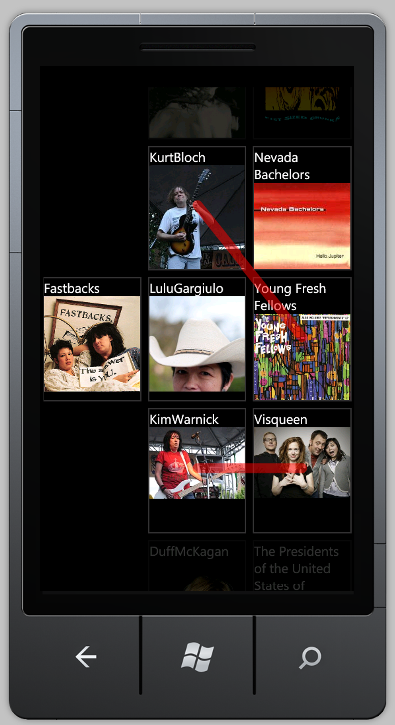
\includegraphics[width=1.6in]{images/bab}}
\subfigure[Band relationship]{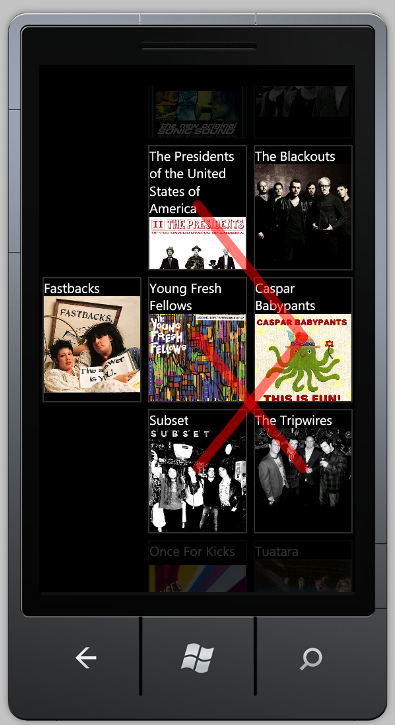
\includegraphics[width=1.6in]{images/bbb}}
\subfigure[Interactive reordering with images dimmed when not related.]{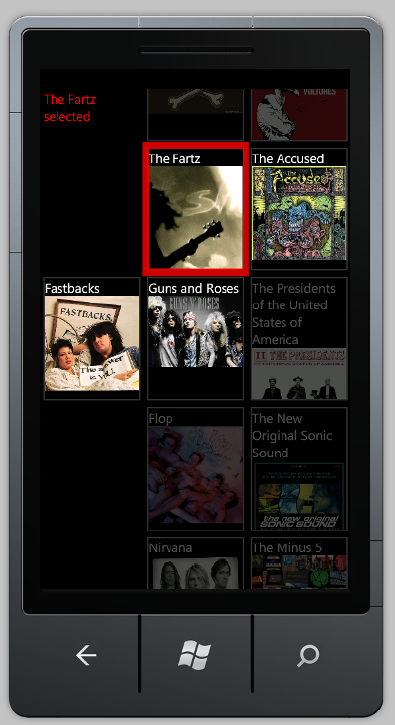
\includegraphics[width=1.6in]{images/fartz_reordering}}
\caption{Applying \textit{GraphTiles} to Seattle's music band data.}
\label{fig:musicband}
\end{figure*}


To confirm that \textit{GraphTiles} supported imprecise search well, we performed an experiment comparing it to a standard mobile information interface. We expected that the specialized \textit{GraphTiles} interface would allow users to perform imprecise search more quickly than an interface supporting the full continuum of information-seeking.

As a typical mobile information interface, we chose the IMDb mobile web app. An imprecise search making use of IMDb is often similar to this: a user wants to recommend a movie to a friend, but cannot remember the name of that movie, nor the name of any actors in that movie. This makes using standard search interfaces somewhat difficult. They do however know that one of the actors in the movie they want to recommend was also in a different movie they can name. They navigate from movie to actor to movie. We focused on answering imprecise queries of that nature. 

Figure \ref{fig:teaser} shows a comparison of the visuals used in \textit{GraphTiles} and IMDb's mobile website (\url{http://m.imdb.com}) to answer movie-person-movie (MPM) queries of this type, as well as person-movie-person (PMP) \textit{QueryTypes}.\\\\


\subsection{Method}

Our experiment had $20$ participants, all of them employees at a large corporate research center.  We obtained informed consent from the participants, and asked them to read the instructions for the experiment. We then familiarized them with the task using 8 training datasets, two for each combination of link \textit{Interface} and \textit{QueryType}. Participants were free to ask verbal questions during training. Each participant performed $120$ information seeking tasks, each using a different graph neighborhood in the IMDb database, with median size of 115 nodes. On average, they completed all their tasks in one hour.

We used a fully crossed within subjects $2 \times 2$ design. As participants performed the tasks, we systematically altered two variables. \textit{Interface}, or the tool used to access the IMDb information, had two levels: \textit{GraphTiles} and the IMDb web app. \textit{QueryType} had two levels: a movie-person-movie (MPM) query or a person-movie-person (PMP) query. If \textit{QueryType} was MPM, we asked participants to find the person who worked in two given movies. In this case, the central node at the left of the visualization was always a movie. If \textit{QueryType} was PMP, we asked participants to find the movie on which two given people collaborated. In this case, the central node at the left of the visualization was always a person. 

To answer a question, participants typically scrolled in the right column to find the second given person or movie. This reordered the middle column, making it easier to scroll in the middle column to find and select the connecting movie or person. Alternatively, participants could first scroll in the middle column, then select each movie or person there and scroll the reordered right column to find the second given person or movie. However, participants quickly learned that the right-first approach was more efficient: it took advantage of faceted search to require only one switch between the right and middle columns, while the middle-first approach ignored the provided faceted search parameter and required several switches.

\textit{GraphTiles} displayed link lines and used interactive reordering. Every participant performed $30$ trials with each of the $2 \times 2 = 4$ experimental treatments. We grouped trials by \textit{Interface} into two blocks of $60$ trials each. Thus participants performed all trials with the current \textit{Interface} before moving on to the next. To combat the effects of fatigue and learning, we used complete counterbalancing across participants: half of them performed the \textit{GraphTiles} block first, the other half the web app block first. Within each of these blocks, we randomly ordered the levels of \textit{QueryType}. We randomized the order of graph neighborhoods without replacement, so that each participant saw each neighborhood exactly once.

\subsubsection{Apparatus}

We implemented \textit{GraphTiles} on three Samsung SGH-i917 phones running Windows Phone 7.5, with an AMOLED display and a full capacitive touch screen. The monitor used to display questions was a $1920 \times 1200$ pixel Dell 24''. Participants interacted with the visualization on a phone by scrolling with a swipe gesture or selecting nodes with a long tap.

We generated our IMDb graph neighborhoods using the official IMDb API (\url{http://www.imdb.com/interfaces}), obtaining a large cross section of its database (approximately 3GB in size). We then randomly selected 60 nodes within the IMDb graph describing well-known actors (supporting PMP queries), and 60 nodes describing well-known movies (supporting MPM queries). We then sampled the two-link neighborhood around each actor (PMP) node by adding the top movies linked to it as indicated by IMDb's own API call; and then for each of those top movies, adding its top actors, again as indicated by IMDb's API call. We created two-link neighborhoods around movie (MPM) nodes similarly. The number of top movies returned by IMDb's API was generally much lower than the number of top actors. 


\subsection{Results}

All participants performed all trials correctly, so we report only completion times here. We tested significance using a two-factor repeated measures ANOVA. Only the two single variable effects were significant; they did not interact. 

When using \textit{GraphTiles}, participants were significantly ($F(1,19)=2291.833$, $p<0.001$) faster than when using the IMDb web app. Average completion time with \textit{GraphTiles} was 18.2s ($\sigma =5.27$), while with IMDb web app, it was 31.5s ($\sigma = 5.26$).

Although its effect was significant ($F(1,19)=11.27$, $p<0.005$), \textit{QueryType}'s effect was not meaningful. The difference in completion times when participants looked for movies rather than persons was 0.6s: (25.0s for movies, 24.4s for persons). The likely explanation for this effect was the consistent differences in MPM vs. PMP neighborhoods.



\subsection{Discussion}

Results in fact exceeded our expectations, with \textit{GraphTiles} users were almost twice as fast as when using the IMDb web app. There are two explanations for \textit{GraphTiles}'s superior performance. First and most important, the faceted search implemented in \textit{GraphTiles} reduced the number of actions users had to take. By first selecting both people or both movies, users could display only the movies or people connecting them. In contrast, IMDb did not implement faceted search, and required users to examine a much larger set of possibly connecting movies or people. Second, \textit{GraphTiles} had several visual advantages. It was a more effective overview: rather than requiring interaction to reveal information two links away (\textit{i.e.} other people in the first person's movies, or other movies in which the cast of the first movie acted), it displayed at least some of them immediately. \textit{GraphTiles} was also less cluttered, without the ads and tertiary information IMDb contains. Finally, \textit{GraphTiles} was less textual than IMDb, and perceptual research consistently shows that visual information is more rapidly understood than text.

Although the degree of \textit{GraphTiles}'s superiority was surprising, that superiority itself was not. \textit{GraphTiles} was designed specifically for imprecise search; IMDb is a more general tool. What remains to be seen is whether or not a single interface can support the full continuum of search generality well. Future work might also attempt to extend our results with other and more types of imprecise search, and by examining the performance of \textit{GraphTiles} with general and precise search.
